\chapter{光照(Lighting)}
\begin{flushleft}
考虑图\ref{fig:8-1}。 在左边我们有一个没有照明的球体,在右边,我们有一个点亮的球体。 正如你所看到的,左边的球体看起来很平坦——也许它根本不是一个球体,而只是一个2D圆圈! 另一方面,右侧的球体确实看起来是3D——照明和阴影有助于我们对物体的固体形状和体积的感知。 事实上,我们对世界的视觉感知取决于光线及其与材料的相互作用,因此,产生逼真场景的大部分问题都与物理上精确的照明模型有关。
\end{flushleft}

\begin{figure}[h]
    \label{fig:8-1}
    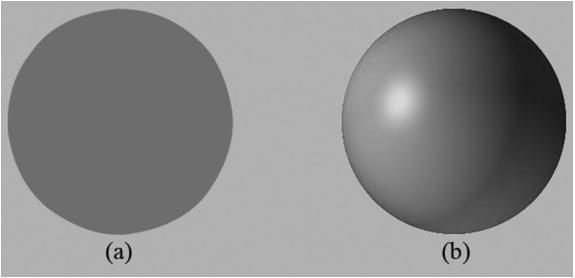
\includegraphics[width=\textwidth]{8-1}
    \centering
    \caption{(a)未点亮的球体看起来是2D。(b)点亮的球体看起来是3D。}
\end{figure}

\begin{flushleft}
当然,一般来说,模型越准确,计算成本越高; 因此,必须在现实主义和速度之间达成平衡。 例如,用于电影的3D特殊FX场景可以比游戏更复杂并且使用非常逼真的照明模型,因为电影的帧是预渲染的,因此它们可以花费数小时或数天来处理帧。 另一方面,游戏是实时应用程序,因此,帧需要以每秒至少30帧的速率绘制。\\
请注意,本书中解释和实现的照明模型很大程度上基于[Möller08]中描述的模型。\\
~\\
{\large Objectives:}
\begin{itemize}
    \item 了解灯光和材料之间的相互作用
    \item 了解局部照明和全局照明之间的差异
    \item 了解我们如何在数学上描述表面上的一个点“朝向”的方向,以便我们可以确定入射光照射到表面的角度
    \item 学习如何正确转换法向量
    \item 能够区分环境光,漫反射光和镜面光
    \item 了解如何实现定向灯,指示灯和聚光灯
    \item 通过控制衰减参数来了解如何根据深度改变光强度
\end{itemize}
\end{flushleft}

%------- 8.1 ---------------
\section{光与材质的相互作用(Light And Meterial Interaction)}
\begin{flushleft}
使用灯光时,我们不再直接指定顶点颜色; 相反,我们指定材质和灯光,然后应用光照方程式,根据光/材料相互作用计算我们的顶点颜色。 这样可以使对象更加逼真地着色(再次比较图\ref{fig:8-1}a和\ref{fig:8-1}b)。\\
可以将材质视为确定光如何与对象表面相互作用的属性。 比如表面反射和吸收的光的颜色,表面下材料的折射率,表面的光滑程度以及表面的透明度。 通过指定材质属性,我们可以模拟不同类型的真实世界表面,如木材,石材,玻璃,金属和水。\\
在我们的模型中,光源可以发出各种强度的红色,绿色和蓝色光; 通过这种方式,我们可以模拟许多浅色。 当光从光源向外传播并与物体碰撞时,一些光可能被吸收而一些光可能被反射(对于透明物体,例如玻璃,一些光线穿过介质,但我们不考虑这里的透明度)。 反射光现在沿着其新的路径行进并且可能撞击其他物体,其中一些光再次被吸收和反射。 在完全吸收之前,光线可能会撞击许多物体。 据推测,一些光线最终会进入眼睛(见图\ref{fig:8-2})并撞击视网膜上的光受体细胞(称为视锥细胞和视杆细胞)。\\
\end{flushleft}

\begin{figure}[h]
    \label{fig:8-2}
    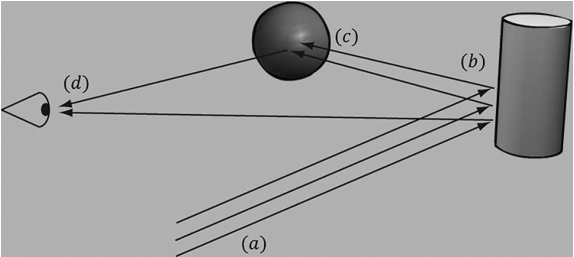
\includegraphics[width=\textwidth]{8-2}
    \centering
    \caption{(a)入射白光的通量。(b)光线照射到圆柱体上,一些光线被吸收,其他光线散射到眼睛和球体上。(c)从圆筒向球体反射的光被再次吸收或反射并进入眼睛。(d)眼睛接收入射光,确定眼睛看到的是什么。}
\end{figure}

\begin{flushleft}
根据三色理论(见[Santrock03]),视网膜含有三种光受体,每种受体对红光,绿光和蓝光敏感(有一些重叠)。 入射的RGB光根据光的强度对其相应的光接收器产生不同强度的刺激。 当光受体受到刺激(或不被刺激)时,神经冲动沿着视神经向大脑发送,大脑基于光受体的刺激在大脑中产生图像。 (当然,如果你闭上/遮住眼睛,受体细胞就不会受到任何刺激,大脑会将其记录为黑色。)\\

例如,再次考虑图\ref{fig:8-2}。假设圆柱体的材料反射75%的红光,75%的绿光,并吸收其余部分,球体反射25%的红光并吸收其余部分。还假设从光源发射纯白光。当光线照射到圆柱体上时,所有的蓝光都被吸收,只有75%的红光和绿光被反射(即,中高强度的黄色)。然后这种光被散射——其中一些光进入眼睛,一些光线向球体传播。进入眼睛的部分主要刺激红色和绿色锥形细胞达到半高度;因此,观察者将圆柱视为半亮的黄色阴影。现在,其他光线向球体射出并撞击它。球体反射25%的红光并吸收其余部分;因此,稀释的入射红光(中高强度红色)被进一步稀释并反射,并且所有进入的绿光被吸收。这剩余的红光然后进入眼睛并较低程度地刺激红锥细胞。因此,观察者将球体视为深红色。\\
我们(和大多数实时应用)在本书中采用的照明模型称为局部照明模型。 使用局部模型,每个对象独立于另一个对象被点亮,并且在光照过程中仅考虑从光源直接发射的光(即,从其他场景对象反弹以击中当前被点亮的对象的光是忽略的)。 图\ref{fig:8-3}显示了该模型的结果。
\end{flushleft}

\begin{figure}[h]
    \label{fig:8-3}
    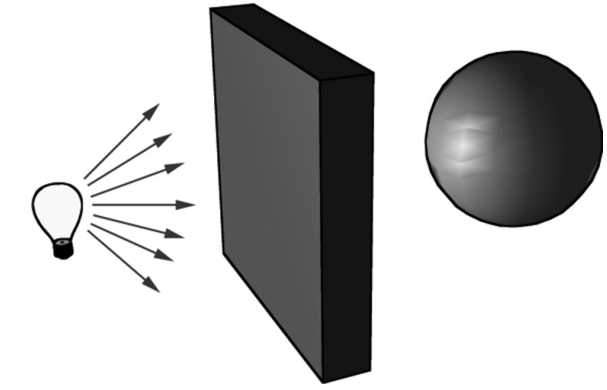
\includegraphics[width=\textwidth]{8-3}
    \centering
    \caption{在物理上,墙壁阻挡了灯泡发出的光线,并且球体位于墙壁的阴影中。 然而,在局部照明模型中,球体被照亮,好像墙壁不存在一样。}
\end{figure}

\begin{flushleft}
另一方面,全局照明通过不仅考虑从光源直接发射的光而且还考虑从场景中的其他物体反弹的间接光来模拟光物体。 这些被称为全局照明模型,因为它们在照亮对象时会考虑全局场景中的所有内容。 对于实时游戏而言,全局照明模型通常过于昂贵(但非常接近于生成逼真的场景)。 寻找近似全局照明的实时方法是一个正在进行研究的领域; 例如,参见\href{http://on-demand.gputechconf.com/gtc/2014/presentations/S4552-rt-voxel-based-global-illumination-gpus.pdf}{\textcolor{linkColor}{voxel global illumination}}。 其他流行的方法是预先计算静态对象(例如,墙壁,雕像)的间接照明,然后使用该结果来近似动态对象的间接照明(例如,移动游戏角色)。\\
\end{flushleft}

%------- 8.2 ---------------
\section{法向量(Normal Vectors)}
\begin{flushleft}
面法线(face normal)是描述多边形正面朝向的单位矢量(即,它与多边形上的所有点正交); 见图\ref{fig:8-4}a。 表面法线是与表面上的点的切平面正交的单位矢量; 见图\ref{fig:8-4}b。 观察表面法线确定表面上的点“朝向”的方向。\\
\end{flushleft}

\begin{figure}[h]
    \label{fig:8-4}
    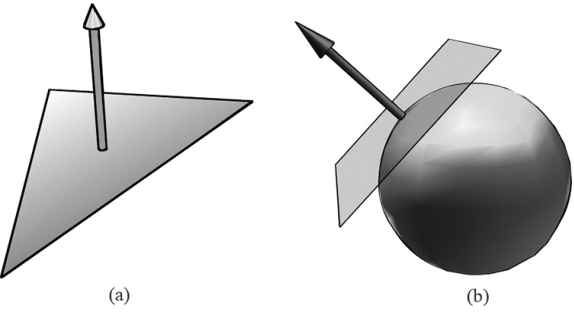
\includegraphics[width=\textwidth]{8-4}
    \centering
    \caption{(a)面部法线与面部上的所有点正交。 (b)表面法线是与表面上的点的切平面正交的矢量。}
\end{figure}

\begin{figure}[h]
    \label{fig:8-5}
    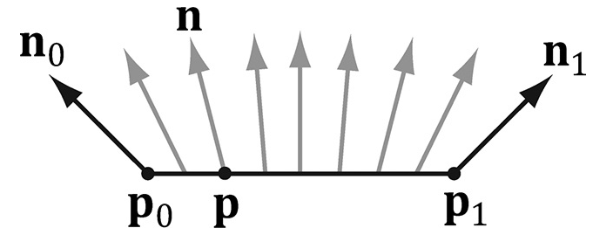
\includegraphics[width=\textwidth]{8-5}
    \centering
    \caption{顶点法线$n_{0}$和$n_{1}$在段顶点$p_{0}$和$p_{1}$处定义。 通过在顶点法线之间进行线性插值(加权平均),找到线段内部的点$p$的法向量$n$; 也就是说,$p=p_{0}+t(p_{1}-p_{0})$,其中$t$代表$p_{0}p$与$p_{0}p_{1}$的比例,则$p$的法线$n=n_{0} + t(n_{1}-n_{0})$。尽管为了简单起见我们在线段上表现了正常插值,但这个想法可以直观地应用在3D三角形上。}
\end{figure}

\begin{flushleft}
对于光照计算,我们需要在三角形网格表面上的每个点处的曲面法线,以便我们可以确定光线照射到网格曲面上的点的角度。 为了获得曲面法线,我们仅在顶点处指定曲面法线(所谓的顶点法线)。 然后,为了在三角形网格的表面上的每个点处获得近似的表面法线,这些顶点法线将在光栅化期间在三角形上插值(回忆5.10.3节并参见图\ref{fig:8-5})。\\
~\\
NOTICE: 对每个像素的法线和光照计算进行插值称为像素照明或phong照明。 一种较便宜但不太精确的方法是每个顶点进行照明计算。 然后,从顶点着色器输出每顶点光照计算的结果,并在三角形的像素上进行插值。 将像素着色器移动到顶点着色器的计算是质量方面的常见性能优化,有时视觉差异非常小,使得这种优化非常有吸引力。\\
\end{flushleft}

%------- 8.2.1 ---------------
\subsection{计算法向量(Computing Normal Vectors)}
\begin{flushleft}
为了找到三角形$p_{0}$,$p_{1}$,$p_{2}$的面法线,我们首先计算位于三角形边缘的两个向量:\\
\end{flushleft}

\begin{align*}
u=p_{1}-p_{0}\\
v=p_{2}-p_{0}
\end{align*}

\begin{flushleft}
然后,其面法向量为:\\
\end{flushleft}

\begin{align*}
n=\frac{u\times v}{||u\times v||}
\end{align*}

\begin{flushleft}
下面是一个函数,用于计算三角形三个顶点的三角形正面(5.10.2节)的面法线。\\
\end{flushleft}

\begin{lstlisting}
XMVECTOR ComputeNormal(FXMVECTOR p0, FXMVECTOR p1, FXMVECTOR p2)
{
    XMVECTOR u = p1 - p0;
    XMVECTOR v = p2 - p0;
    return XMVector3Normalize(XMVector3Cross(u,v));
}
\end{lstlisting}

\begin{figure}[h]
    \label{fig:8-6}
    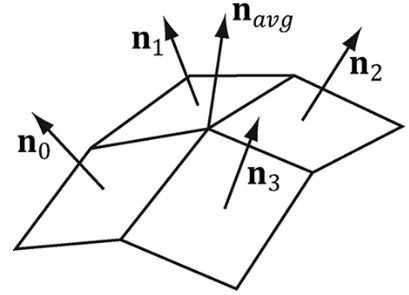
\includegraphics[width=\textwidth]{8-6}
    \centering
    \caption{中间顶点由相邻的四个多边形共享,因此我们通过平均四个多边形面法线来近似中间顶点法线。}
\end{figure}

\begin{flushleft}
对于可微分的表面,我们可以使用微积分来找到曲面上的法线。 不幸的是,三角形网格不可区分。 通常应用于三角形网格的技术称为顶点法线平均(vetex normal averaging)。 网格中的顶点法线$n$或任意顶点$v$是通过平均共享顶点$v$的网格中每个多边形的面法线来找到的。例如,在图\ref{fig:8-6}中,网格中的四个多边形因此共享顶点$v$, $v$的顶点法线由下式给出:\\
\end{flushleft}

\begin{align*}
n_{avg}=\frac{n_{0}+n_{1}+n_{2}+n_{3}}{||n_{0}+n_{1}+n_{2}+n_{3}||}
\end{align*}

\begin{flushleft}
在上面的例子中,我们不需要除以4,就像我们在典型的平均值中那样,因为我们将结果标准化。 还要注意,可以构建更复杂的平均方案; 例如,可以使用加权平均值,其中权重由多边形的面积确定(例如,具有较大区域的多边形比具有较小区域的多边形具有更多权重)。\\
以下伪代码显示了如何在给定三角形网格的顶点和索引列表的情况下实现此平均:\\
\end{flushleft}

\begin{lstlisting}
// Input:
// 1. An array of vertices (mVertices). Each vertex has a
// position component (pos) and a normal component (normal).
// 2. An array of indices (mIndices).
// For each triangle in the mesh:
for(UINT i = 0; i < mNumTriangles; ++i)
{
    // indices of the ith triangle
    UINT i0 = mIndices[i*3+0];
    UINT i1 = mIndices[i*3+1];
    UINT i2 = mIndices[i*3+2];

    // vertices of ith triangle
    Vertex v0 = mVertices[i0];
    Vertex v1 = mVertices[i1];
    Vertex v2 = mVertices[i2];

    // compute face normal
    Vector3 e0 = v1.pos - v0.pos;
    Vector3 e1 = v2.pos - v0.pos;
    Vector3 faceNormal = Cross(e0, e1);

    // This triangle shares the following three vertices,
    // so add this face normal into the average of these
    // vertex normals.
    mVertices[i0].normal += faceNormal;
    mVertices[i1].normal += faceNormal;
    mVertices[i2].normal += faceNormal;
}
// For each vertex v, we have summed the face normals of all
// the triangles that share v, so now we just need to normalize.
for(UINT i = 0; i < mNumVertices; ++i)
    mVertices[i].normal = Normalize(&mVertices[i].normal));
\end{lstlisting}

%------- 8.2.2 ---------------
\subsection{转换法向量(Transforming Normal Vectors)}
\begin{flushleft}
考虑图\ref{fig:8-7}a,其中我们具有与法向量$n$正交的切向量$u=v_{1}-v_{0}$。 如果我们应用非均匀缩放变换$A$,我们从图\ref{fig:8-7}b中看到,变换的切向量$uA=v_{1}A-v_{0}A$不与变换的法向量$nA$保持正交。
\end{flushleft}

\begin{figure}
\label{fig:8-7}
\begin{subfigure}{1\textwidth}
  \centering
  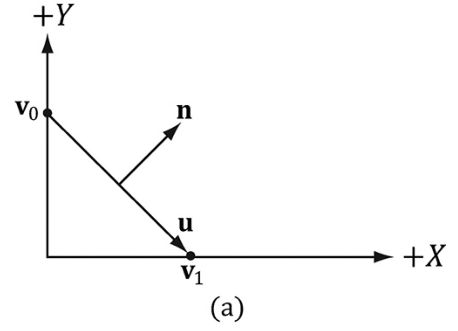
\includegraphics[width=1\linewidth]{8-7-a}
\end{subfigure}
\begin{subfigure}{1\textwidth}
  \centering
  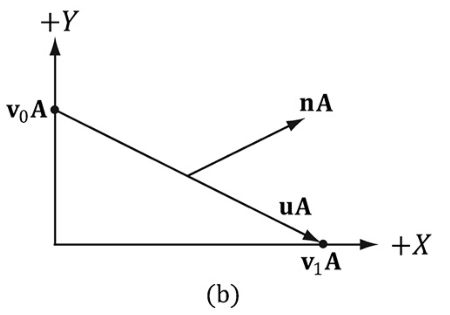
\includegraphics[width=1\linewidth]{8-7-b}
\end{subfigure}
\begin{subfigure}{1\textwidth}
  \centering
  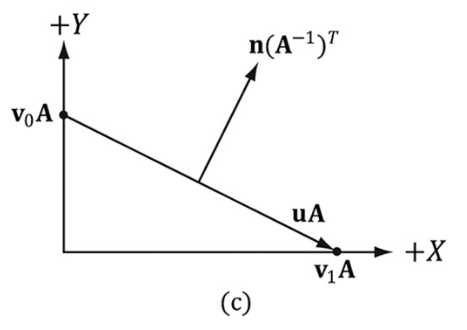
\includegraphics[width=1\linewidth]{8-7-c}
\end{subfigure}
\caption{(a)转变前的表面法线。(b)在x轴上缩放2个单位后,法线不再与表面正交。 (c)通过缩放变换的逆转置正确地变换的表面法线。}
\end{figure}

\begin{flushleft}
所以我们的问题是:给定转换矩阵$A$转换点和向量(非正态),我们想找到一个转换矩阵$B$,使得转换的切线向量与转换的法向量正交(即 $uA\cdot nB = 0$)。 要做到这一点,首先从我们知道的东西开始:我们知道法向量$n$与切向量$u$正交:\\
\end{flushleft}

\begin{tabular}{|p{5em}|p{35em}|} 
\hline
$u\cdot n=0$ & 切线向量与法向量正交\\ 
\hline
$un^{T}=0$ & 将点积重写为矩阵乘法\\ 
\hline
$u(AA^{-1})n^{T}=0$ & 插入单位矩阵$I=AA^{-1}$\\
\hline 
$(uA)(A^{-1}n^{T})=0$ & 矩阵乘法结合律\\
\hline 
$(uA)(((A^{-1}n^{T})^{T})^{T})=0$ & 矩阵转置性质:$(A^{T})^{T}=A$\\
\hline 
$(uA)((n(A^{-1})^{T})^{T})=0$ & 矩阵转置性质:$(AB^{T})^{T}=B^{T}A^{T}$\\
\hline 
$uA\cdot n(A^{-1})^{T}=0$ & 将矩阵乘法重写为点积\\ 
\hline
$uA\cdot nB=0$ & 经B转换的法向量与经A转换的法向量正交\\ 
\hline
\end{tabular}

\begin{flushleft}
因此,$B=(A^{-1})^{T}$(A的逆转置)在转换法向量时起作用,使得它们垂直于其相关的变换切线向量$uA$。\\

注意,如果矩阵是正交的(正交矩阵$(A^{T}=A^{-1})$),则$B=(A^{-1})^{T}=(A^{T})^{T}=A$; 也就是说,我们不需要计算逆转置,因为A在这种情况下完成了工作。 总之,当通过非均匀或剪切变换转换法向量时,请使用逆转置。\\
我们在 MathHelper.h 中实现了一个辅助函数来计算逆转换:\\
\end{flushleft}

\begin{lstlisting}
static XMMATRIX InverseTranspose(CXMMATRIX M)
{
    XMMATRIX A = M;
    A.r[3] = XMVectorSet(0.0f, 0.0f, 0.0f, 1.0f);
    XMVECTOR det = XMMatrixDeterminant(A);
    return XMMatrixTranspose(XMMatrixInverse(&det, A));
}
\end{lstlisting}

\begin{flushleft}
我们清除矩阵中的任何平移转换,因为我们使用逆转置来转换向量,并且转换仅适用于点。 但是,根据 3.2.1 节,我们知道为向量设置$w=0$(使用齐次坐标)可以防止向量被平移变换修改。 因此,我们不应该将矩阵中的平移归零。 问题是如果我们想要连接逆转置和不包含非均匀缩放的另一个矩阵,比如视图矩阵$(A^{-1})^{T}V$,$(A^{-1})^{T}$的第四列中的转置平移"泄漏"(leaks)到矩阵乘法运算导致错误。因此,我们将平移归零以作为预防措施以避免此错误。 正确的方法是通过以下方式转换法线:$((AV)^{-1})^{T}$。 下面是缩放和平移矩阵的示例,以及第四列不是$[0,0,0,1]^{T}$的逆转置看起来是什么样的:\\
\end{flushleft}

\begin{align*}
A&=
\begin{bmatrix}
1 & 0 & 0 & 0\\
0 & 0.5 & 0 & 0\\
0 & 0 & 0.5 & 0\\
1 & 1 & 1 & 1
\end{bmatrix}\\
(A^{-1})^{T}&=
\begin{bmatrix}
1 & 0 & 0 & -1\\
0 & 2 & 0 & -2\\
0 & 0 & 2 & -2\\
0 & 0 & 0 & 1
\end{bmatrix}
\end{align*}

\begin{flushleft}
NOTICE: 即使使用逆转置变换,法向量也可能失去单位长度; 因此,它们可能需要在转换后重新规范化。
\end{flushleft}

%------- 8.3 ---------------
\section{照明中的重要向量(Important Vectors In Lighting)}
\begin{flushleft}
在本节中,我们总结了一些与照明有关的重要向量。参考图\ref{fig:8-8},$E$是眼睛位置,我们正在考虑眼睛沿着由单位向量$v$定义的位置线看到的点$p$。在点$p$ 处,表面具有法向量$n$,并且该点被一个入射方向$I$的光线击中。光向量$L$是朝向撞击表面点的光线的相反方向的单位矢量。虽然使用光传播方向可能更直观,但对于光照计算,我们使用光向量$L$;特别地,为了计算朗伯余弦定律(Lambert’s Cosine Law),向量$L$用于计算$L\cdot n=cos\Theta_{i}$,其中$\Theta_{i}$是$L$和$n$之间的角度。反射向量$r$是关于表面法线$n$的入射光向量的反射。视图向量(或眼睛向量)$v$=标准化$(E-p)$是从表面点$p$到眼点$E$的单位向量,其定义从眼睛到被观察表面上的点的位置线。有时我们需要使用矢量$-v$,它是从眼睛到表面上我们正在计算光照的点的单位向量。\\
\end{flushleft}

\begin{figure}[h]
    \label{fig:8-8}
    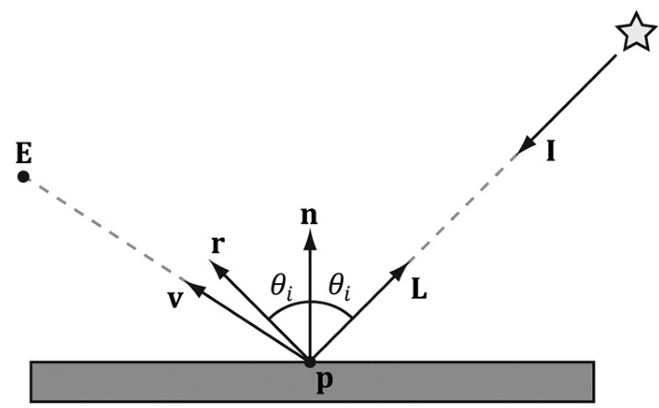
\includegraphics[width=\textwidth]{8-8}
    \centering
    \caption{光照计算中涉及到的重要向量}
\end{figure}

\begin{flushleft}
反射向量由下式给出:$r=I-2(n\cdot I)n$; 见图\ref{fig:8-9}。 (假设$n$是单位向量。)但是,我们实际上可以使用HLSL内部反射函数在着色器程序中为我们计算$r$。
\end{flushleft}

\begin{figure}[h]
    \label{fig:8-9}
    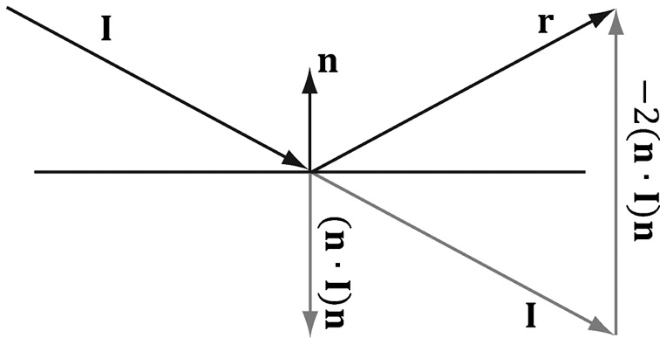
\includegraphics[width=\textwidth]{8-9}
    \centering
    \caption{反射几何}
\end{figure}

%------- 8.4 ---------------
\section{朗伯余弦定律(Lambert’s Cosine Law)}
\begin{flushleft}
我们可以将光视为在某个方向上穿过空间的光子集合。每个光子携带一些(光)能量。 每秒发射的(光)能量的量称为辐射通量。 每个区域的辐射通量密度(称为辐照度)很重要,因为这将决定表面上的区域接收多少光(它对眼睛看起来有多亮)。 粗略说,我们可以将辐照度视为撞击表面上的区域的光量,或者通过空间中的假想区域的光量。\\

正面撞击表面的光(即,光向量$L$等于法线向量$n$)比以一定角度掠过表面的光更强烈。考虑具有横截面积$A_{1}$的小光束,其中辐射通量$P$穿过它。 如果我们将这个光束瞄准正面(图\ref{fig:8-10}a),则光束照射到表面上的区域$A_{1}$,$A_{1}$处的辐照度为$E_{1}=P/A_{1}$。 现在假设我们旋转光束使其以一定角度撞击表面(图\ref{fig:8-10}b),然后光束覆盖较大的区域$A_{2}$,并且照射该区域的辐照度为$E_{2}=P/A_{2}$。 通过三角函数,$A_{1}$和$A_{2}$通过以下方式关联:\\
\end{flushleft}

\begin{align*}
cos\Theta = \frac{A_{1}}{A_{2}}\Rightarrow \frac{1}{A_{2}}=\frac{cos\Theta}{A_{1}}
\end{align*}

\begin{flushleft}
所以,\\
\end{flushleft}

\begin{align*}
E_{2}=\frac{P}{A_{2}}=\frac{P}{A_{1}}cos\Theta=E_{1}cos\Theta=E_{1}(n\cdot L)
\end{align*}

\begin{figure}[h]
    \label{fig:8-10}
    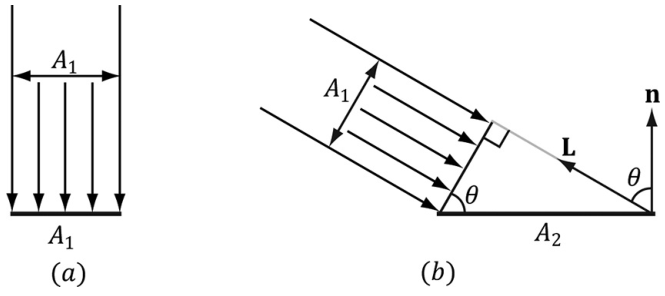
\includegraphics[width=\textwidth]{8-10}
    \centering
    \caption{(a)横截面积为$A_{1}$的光束正面撞击表面。(b)具有横截面面积$A_{1}$的光束以一定角度撞击表面以覆盖表面上的较大区域$A_{2}$,从而将光能扩散到更大的区域上,从而使光看起来“更暗”。}
\end{figure}

\begin{flushleft}
换句话说,辐照度打击区域$A_{2}$等于垂直于被$n\cdot L=cos\Theta$缩放变换的光方向的区域$A_{1}$处的辐照度。 这被称为兰伯特的余弦定律。 为了处理光线照射到背面(导致点积为负)的情况,我们用最大函数限制结果:\\
\end{flushleft}

\begin{align*}
f(\Theta)=max(cos\Theta,0)=max(L\cdot n, 0)
\end{align*}

\begin{flushleft}
图\ref{fig:8-11}显示了$f(\Theta)$的曲线图,以观察 0.0 到 1.0(即0%到100%)的强度如何随θ变化。
\end{flushleft}

\begin{figure}[h]
    \label{fig:8-11}
    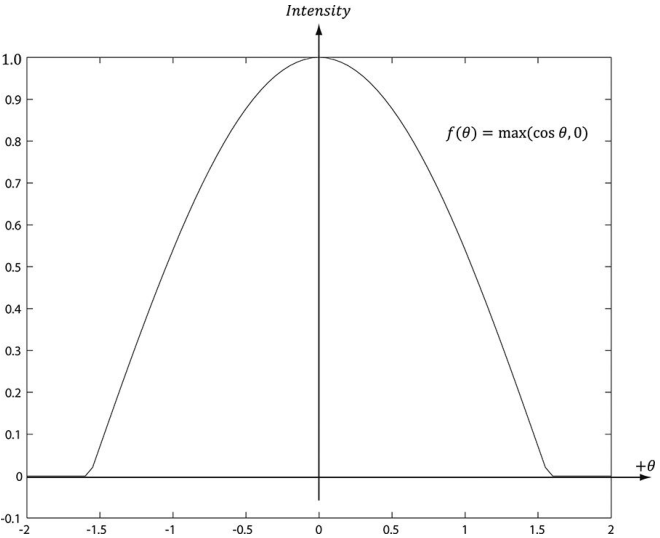
\includegraphics[width=\textwidth]{8-11}
    \centering
    \caption{对于$-2\leq \Theta \leq 2$,函数$f(\Theta)=max(cos\Theta,0)=max(L\cdot n, 0)$的曲线图。注意$\pi /2 \approx 1.57$。}
\end{figure}

%------- 8.5 ---------------
\section{漫射照明(Diffuse Lighting)}
\begin{flushleft}
考虑不透明物体的表面,如图\ref{fig:8-12}所示。当光线照射到表面上的某个点时,一些光线会进入物体内部并与表面附近的物质相互作用。光线会在内部反射,其中一些会被吸收,剩下的部分会向各个方向散射出来;这称为漫反射。为简化起见,我们假设光线在光线进入的同一点散射出来。吸收和散射的量取决于材料;例如,木材,泥土,砖块,瓷砖和灰泥会不同地吸收/散射光线(这就是材料看起来不同的原因)。我们对这种光/材料相互作用近似建模,规定光在表面上方的所有方向上均匀散射;因此,无论视点(眼睛位置)如何,反射光都会到达眼睛。因此,我们不需要考虑该视点(即,漫射照明计算是视点无关的),并且无论视点如何,表面上的点的颜色总是看起来相同。\\
\end{flushleft}

\begin{figure}[h]
    \label{fig:8-12}
    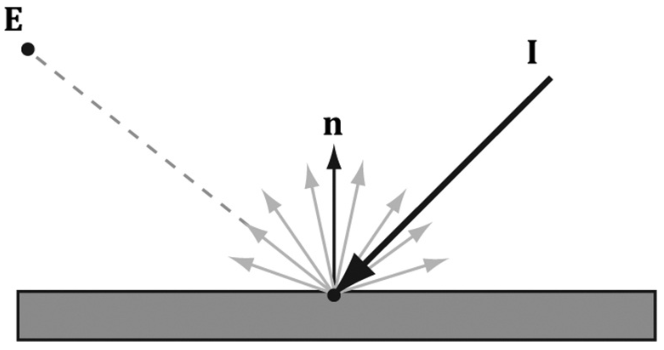
\includegraphics[width=\textwidth]{8-12}
    \centering
    \caption{当撞击漫射表面时,入射光在每个方向上均匀地散射。 这个想法是光进入介质的内部并在表面下散射。 一些光将被吸收,剩余的光会从表面散射回来。 因为很难对这种次表面散射进行建模,所以我们假设重新发射的光在光进入的点附近在表面上方的所有方向上均匀地散射出来。}
\end{figure}

\begin{flushleft}
我们将漫射照明的计算分为两部分。 对于第一部分,我们指定浅色和漫反射色。 漫反射率指定了由于漫反射而表面反射的入射光量(通过节能,未反射的量被材料吸收)。 这是通过分量色彩乘法处理的(因为光可以着色)。 例如,假设表面上的某些点反射50%的入射红光,100%的绿光和75%的蓝光,并且入射光的颜色是80%强度的白光。 也就是说,入射光量由$B_{L}=(0.8,0.8,0.8)$给出,漫反射率由$m_{d}=(0.5,1.0,0.75)$ 给出; 那么从该点反射的光量由下式给出:\\
\end{flushleft}

\begin{align*}
c_{d}=B_{L}\bigotimes m_{d}=(0.8,0.8,0.8)\bigotimes (0.5,1.0,0.75)=(0.4,0.8,0.6)
\end{align*}

\begin{flushleft}
请注意,漫反射率反射率分量必须在0.0到1.0的范围内,以便它们描述反射光的分数。\\
但是,上述公式并不完全正确。 我们仍然需要引入Lambert的余弦定律(它根据表面法线和光向量之间的角度控制表面接收的原始光的多少)。 设$B_{L}$表示入射光量,$m_{d}$ 是漫反射率颜色,$L$是光向量,$n$是表面法线。 然后,一个点反射的漫射光量由下式给出:\\
\end{flushleft}

\begin{align*}\tag{eq.8.1}\label{eq.8.1}
c_{d}=max(L\cdot n, 0)\cdot B_{L}\bigotimes m_{d}
\end{align*}

%------- 8.6 ---------------
\section{环境照明(Ambient Lighting)}
\begin{flushleft}
如前所述,我们的照明模型没有考虑从场景中的其他物体反弹的间接光。 然而,我们在现实世界中看到的很多光是间接的。 例如,连接到房间的走廊可能不在房间的直接线路中,房间内有光源,但是灯光从房间的墙壁反弹,有些可能会进入走廊,从而使其变亮一点点。 作为第二个例子,假设我们坐在桌子上有茶壶的房间里,房间里有一个光源。 只有茶壶的一侧位于光源的直线上; 然而,茶壶的背面不会是完全黑色的。 这是因为一些光线从房间的墙壁或其他物体上散开,最终撞击茶壶的背面。\\
为了解释这种间接光,我们在照明方程中引入了一个环境术语:\\
\end{flushleft}

\begin{align*}\tag{eq.8.2}\label{eq.8.2}
c_{a}=A_{L}\bigotimes m_{d}
\end{align*}

\begin{align*}
颜色$A_{L}$表示表面接收的间接(环境)光的总量,与从光源发出的光不同,这是由于当光从其他表面反弹时发生的吸收。 漫反射率$m_{d}$表示由于漫反射而表面反射的入射光量。 我们使用相同的值来指定表面反射的入射环境光量; 也就是说,对于环境照明,我们正在模拟间接(环境)光的漫反射。 所有环境光都会使物体均匀亮一点 - 根本没有真正的物理计算。 这个想法是,间接光在场景周围散射和反射很多次,以至于它在每个方向上均匀地撞击物体。
\end{align*}

%------- 8.7 ---------------
\section{高光照明(Specular Lighting)}
\begin{flushleft}
我们使用漫射照明来模拟漫反射,其中光进入介质,反射,一些光被吸收,剩余的光在每个方向上从介质中散射出来。 由于菲涅耳效应(Fresnel effect),发生了第二种反射,这是一种物理现象。 当光线到达具有不同折射率的两种介质之间的界面时,一些光被反射,剩余的光被折射(见图\ref{fig:8-13})。 折射率是介质的物理性质,其是真空中的光速与给定介质中的光速之比。 我们将这种光反射过程称为镜面反射,将反射光称为镜面反射光。 镜面光如图\ref{fig:8-14}a所示。
\end{flushleft}

\begin{figure}[h]
    \label{fig:8-13}
    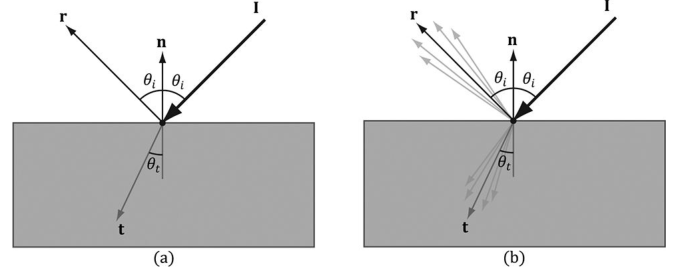
\includegraphics[width=\textwidth]{8-13}
    \centering
    \caption{(a)对于具有法向量$n$的完全平坦的镜子的菲涅耳效应(Frenel eefct)。 入射光$I$被分开,其中一些光在反射方向$r$上反射,并且剩余的光在折射方向$t$上折射到介质中。 所有这些向量都在同一平面上。 反射向量和法线之间的角度总是$θ_{i}$,这与光向量$L=-I$和法线$n$之间的角度相同。 折射向量和$-n$之间的角度$θ_{t}$取决于两种介质之间的折射率,并由斯涅尔定律(Snell's Law)表示。 (b)大多数物体不是完全平坦的镜子,但具有微观粗糙度。 这导致反射和折射的光在反射和折射矢量周围扩散。}
\end{figure}

\begin{flushleft}
如果折射的向量离开介质(从另一侧)并进入眼睛,则该物体看起来是透明的。 也就是说,光线穿过透明物体。 实时图形通常使用alpha混合或后期处理效果来近似透明对象的折射,我们将在本书后面解释。 目前,我们只考虑不透明的对象。\\
对于不透明物体,折射光进入介质并经历漫反射。 因此我们可以从图\ref{fig:8-14}b中看到,对于不透明物体,从表面反射并使其进入眼睛的光量是身体反射(漫射)光和镜面反射的组合。 与漫射光相比,镜面光可能不会进入眼睛,因为它反射在特定方向; 也就是说,镜面反射计算是视点相关的。 这意味着当眼睛在场景周围移动时,它接收的镜面光量将发生变化。\\
\end{flushleft}

\begin{figure}[h]
    \label{fig:8-14}
    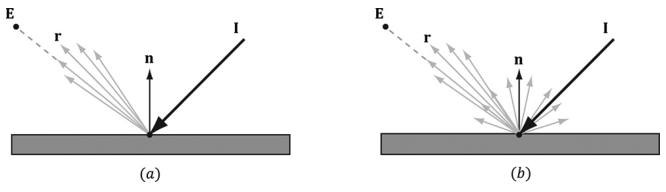
\includegraphics[width=\textwidth]{8-14}
    \centering
    \caption{(a)粗糙表面的镜面光围绕反射向量$r$扩散。 (b)使其进入眼睛的反射光是镜面反射和漫反射的组合。}
\end{figure}

%------- 8.7.1 ---------------
\subsection{菲涅耳效应(Fresnel Effect)}
\begin{flushleft}
让我们考虑具有法向量$n$的平坦表面,该向量将具有不同折射率的两种介质分开。 由于表面处的折射率不连续,当入射光照射到表面时,一些反射离开表面,一些折射到表面(见图\ref{fig:8-13})。 菲涅耳方程在数学上描述了被反射的入射光的百分比,$0\leq R_{F} \leq 1$。通过能量守恒,如果$R_{F}$是反射光的量,则$(1-R_{F})$是折射光的量。 值$R_{F}$是 RGB 向量,因为反射量取决于光的颜色。\\
反射的光量取决于介质(某些材料将比其他材料更具反射性)以及法向量$n$和光向量$L$之间的角度$\Theta_{i}$。由于它们的复杂性,完整的菲涅耳方程通常不用于实时渲染; 相反,使用 Schlick 近似:\\
\end{flushleft}

\begin{align*}
R_{F}(\Theta_{i})=R_{F}(0^{\circ})+(1-R_{F}(0^{\circ}))(1-cos\Theta_{i})^{5} 
\end{align*}

\begin{flushleft}
$R_{F}(0^{\circ})$是介质的特性; 以下是常见材料的一些值[Möller08]:\\
\end{flushleft}

\begin{tabular}{|p{5em}|p{35em}|} 
\hline
介质 & $R_{F}(0^{\circ})$\\ 
\hline
水 & $(0.02,0.02,0.02)$\\ 
\hline
玻璃 & $(0.08,0.08,0.08)$\\ 
\hline
塑料 & $(0.05,0.05,0.05)$\\ 
\hline
金 & $(1.0,0.71,0.29)$\\ 
\hline
银 & $(0.95,0.93,0.88)$\\ 
\hline
铜 & $(0.95,0.64,0.54)$\\ 
\hline
\end{tabular}

\begin{flushleft}
图\ref{fig:8-15}显示了几个不同$R_{F}(0^{\circ})$的 Schlick 近似图。观察的关键是反射量随着$\Theta_{i}\rightarrow 90^{\circ}$的增加而增加。让我们看一个现实世界的例子。考虑图\ref{fig:8-16}。假设我们站在一个相对清澈的水的平静池塘深处几英尺深。如果我们向下看,我们大多看到池塘底部的沙子和岩石。这是因为从环境反射到我们眼睛中的光形成了接近$0.0^{\circ}$的小角度$\Theta_{i}$;因此,反射量低,并且因为节能,折射量高。另一方面,如果我们望向地平线,我们将看到池塘水中的强烈反射。这是因为从进入我们眼睛的环境下来的光形成接近$90.0^{\circ}$的角度$\Theta_{i}$,从而增加了反射量。此行为通常称为菲涅耳效应。简要总结菲涅耳效应:反射光的量取决于材料$R_{F}(0^{\circ})$和法向量与光向量之间的角度。\\
\end{flushleft}

\begin{figure}[h]
    \label{fig:8-15}
    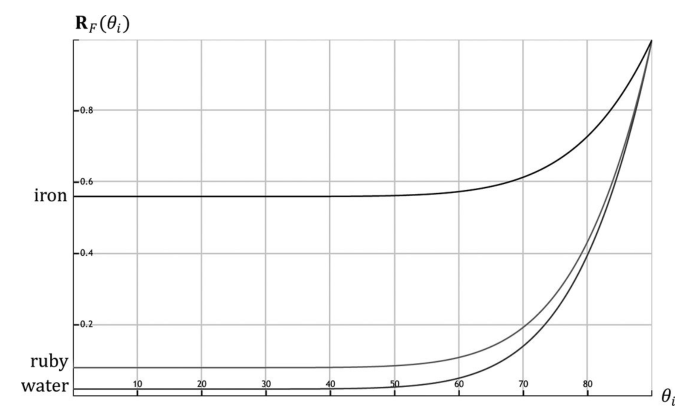
\includegraphics[width=\textwidth]{8-15}
    \centering
    \caption{针对不同材料绘制的Schlick近似值:水,红宝石和铁。}
\end{figure}

\begin{figure}[h]
    \label{fig:8-16}
    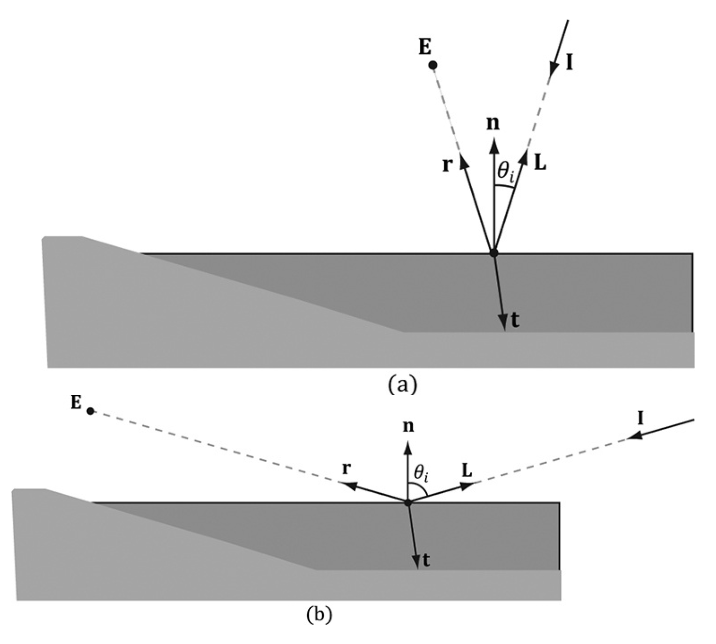
\includegraphics[width=\textwidth]{8-16}
    \centering
    \caption{(a):俯视池塘,反射低,折射高,因为$L$和$n$之间的角度很小。 (b)看向地平线,反射高,折射低,因为$L$和$n$之间的角度接近$90^{\circ}$。}
\end{figure}

\begin{flushleft}
金属吸收透射光[Möller08],这意味着它们不会有人体反射。 然而,金属看起来不是黑色,因为它们具有高$R_{F}(0^{\circ})$值,这意味着即使在$0^{\circ}$附近的小入射角下它们也能反射相当数量的镜面反射光。\\
\end{flushleft}
\clearpage

%------- 8.7.2 ---------------
\subsection{粗糙度(Roughness)}
\begin{flushleft}
现实世界中的反光物体往往不是完美的镜子。 即使物体的表面看起来是扁平的,在微观层面我们也可以认为它具有粗糙度。 参见图\ref{fig:8-17},我们可以认为一个完美的镜子没有粗糙度,它的微法线都与宏观法线的方向相同。 随着粗糙度的增加,微法线的方向偏离宏观法线,导致反射光扩散到镜面波瓣。
\end{flushleft}

\begin{figure}[h]
    \label{fig:8-17}
    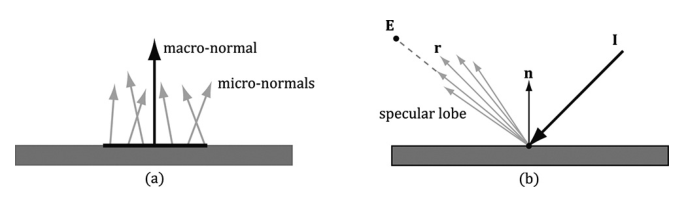
\includegraphics[width=\textwidth]{8-17}
    \centering
    \caption{(a)黑色水平条表示小表面元素的放大。 在微观层面,该区域具有许多微观法线,由于微观水平的粗糙度而瞄准不同的方向。 表面越光滑,微法线与宏观法线的平均值越大; 表面越粗糙,微法线就越偏离宏观法线。(b)这种粗糙度导致镜面反射光扩散。 镜面反射的形状称为镜面反射。 通常,镜面凸角的形状可以根据被建模的表面材料的类型而变化。}
\end{figure}

\begin{flushleft}
为了在数学上模拟粗糙度,我们采用了微平面模型,我们将微观表面建模为一组称为微平面的微小扁平元素; 微法线是微平面的法线。 对于给定的视图$v$和光向量$L$,我们想要知道将$L$反射为$v$的微平面的分数(faction); 换句话说,具有法线$h=$标准化$(L + v)$的微平面的分数(faction); 见图\ref{fig:8-18}。 这将告诉我们有多少光线从镜面反射到眼睛中——将$L$反射到$v$中的微透镜越多,眼睛看到的镜面反射光越亮。
\end{flushleft}

\begin{figure}[h]
    \label{fig:8-18}
    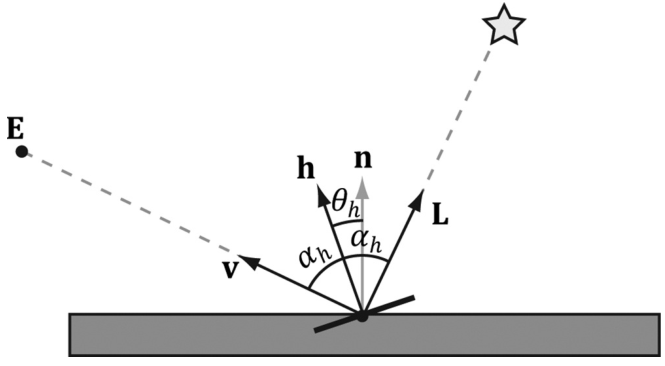
\includegraphics[width=\textwidth]{8-18}
    \centering
    \caption{具有法线$h$的微平面将$L$反射为$v$。}
\end{figure}

\begin{flushleft}
向量$h$被称为中间向量,因为它位于$L$和$v$之间的中间。此外,我们还介绍中间向量$h$和宏观法线$n$之间的角度$\Theta h$。\\

我们定义归一化分布函数$\rho(\Theta_{h})\epsilon [0,1]$来表示具有法线$h$的微平面的分数,其与宏观法线$n$形成角度$\Theta h$。 直观地,我们期望当$\Theta h=0^{\circ}$时$\rho(\Theta_{h})$达到其最大值。 也就是说,我们预计微平面法线偏向宏观法线,并且随着$\Theta h$增加(当$h$偏离微法线$n$时),法线$h$的微平面的比例将减小。 一个流行的可控函数模型$\rho(\Theta_{h})$符合刚才讨论的期望:\\
\end{flushleft}

\begin{align*}
\rho(\Theta_{h})&=cos^{m}(\Theta_{h})\\
&=cos^{m}(n\cdot h)
\end{align*}

\begin{flushleft}
注意,$cos(\Theta h)=(n\cdot h)$提供了向量和单位长度。 图\ref{fig:8-19}显示了各种$m$的$\rho(\Theta_{h})=cos_{h}(\Theta_{h})$。 这里$m$控制粗糙度,代表具有法线$h$的微平面的分数,与宏观法线$n$形成角度$\Theta_{h}$。 随着$m$减小,表面变得更粗糙,并且微平面法线越来越偏离宏观法线。 随着$m$增加,表面变得更平滑,并且微平面法线越来越收敛于宏观法线。
\end{flushleft}

\begin{figure}[h]
    \label{fig:8-19}
    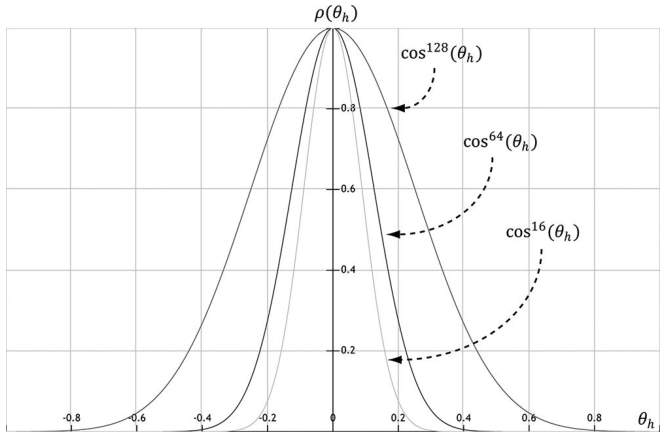
\includegraphics[width=\textwidth]{8-19}
    \centering
    \caption{具有法线$h$的微平面将$L$反射为$v$。}
\end{figure}

\begin{flushleft}
我们可以将$\rho(\Theta_{h})$与归一化因子结合起来,以获得一个基于粗糙度模拟光的镜面反射量的新函数:\\
\end{flushleft}

\begin{align*}
S(\Theta_{h})&=\frac{m+8}{8}cos^{m}(\Theta_{h})\\
&=\frac{m+8}{8}(n\cdot h)^{m}
\end{align*}

\begin{flushleft}
图\ref{fig:8-20}显示了该函数的各种$m$。 像以前一样,$m$控制粗糙度,但我们增加了$\frac{m+8}{8}$归一化因子,以便保存光能; 它基本上控制了图\ref{fig:8-20}中曲线的高度,因此当镜面波瓣变宽或变窄时,整体光能得以保存。 对于较小的$m$,表面较粗糙,镜面波瓣随着光能量的扩散而变宽; 因此,我们预计,由于能量已经分散,镜面高光会变暗。 另一方面,对于更大的$m$,表面更光滑并且镜面波瓣更窄; 因此,我们预计,由于能量集中,镜面高光更加明亮。 几何上,$m$控制镜面波瓣的扩散。 要模拟光滑的表面(如抛光金属),您将使用较大的$m$,而对于较粗糙的表面,您将使用较小的$m$。
\end{flushleft}

\begin{figure}[h]
    \label{fig:8-20}
    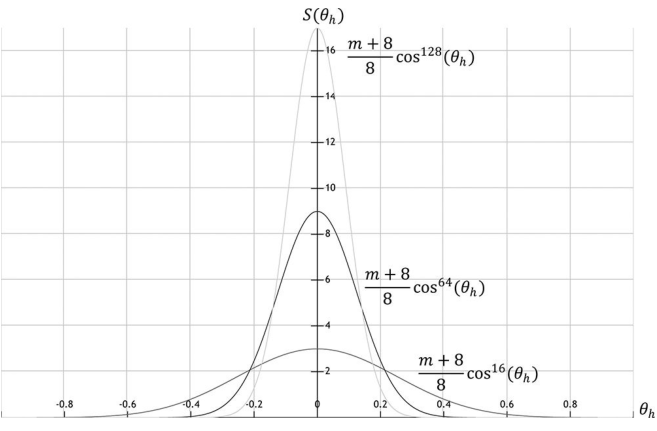
\includegraphics[width=\textwidth]{8-20}
    \centering
    \caption{由粗糙度模拟光的镜面反射的函数。}
\end{figure}

\begin{flushleft}
总结本节,让我们结合菲涅耳反射和表面粗糙度。 我们正在尝试计算反射到视图方向$v$的光量(见图\ref{fig:8-18})。 回想一下,具有法线$h$的微平面将光反射到$v$中。令$\alpha_{h}$是光向量和半向量$h$之间的角度,然后$R_{F}(\alpha_{h})$告诉我们由于菲涅耳效应而将$h$反射到$v$中的光量。 由于菲涅耳效应引起的反射光$R_{F}(\alpha_{h})$的量乘以由粗糙度$S(\Theta_{h})$引起的反射光量,得到镜面反射光的量:$(max(L\cdot n,0)\cdot B_{L})$表示撞击我们正在照射的表面点的入射光的量,然后由于粗糙度和菲涅耳效应而镜面反射到眼睛中的$(max(L\cdot n,0)\cdot B_{L})$的分数由下式给出:\\
\end{flushleft}

\begin{align*}\tag{eq.8.3}\label{eq.8.3}
c_{s}=max(L\cdot n, 0)\cdot B_{L}\bigotimes R_{F}(\alpha_{h})\frac{m+8}{8}(n\cdot h)^{m}
\end{align*}

\begin{flushleft}
观察到如果$L\cdot n\leq 0$,则光线照射到我们正在计算的表面背面;因此前侧表面不接收光。
\end{flushleft}

%------- 8.8 ---------------
\section{照明模型回顾(Lighting Model Recap)}
\begin{flushleft}
将所有物质组合在一起,从表面反射的总光量是环境光反射率,漫反射光反射率和镜面反射光的总和:\\
\end{flushleft}

\begin{itemize}
  \item 1.环境光$c_{a}$:模拟由于间接光线而从表面反射的光量。
  \item 2.漫射光$c_{d}$:模拟进入介质内部的光线,散射在表面下方,其中一些光线被吸收,剩余的光线从表面散射回来。 因为很难对这种次表面散射进行建模,所以我们假设重新发射的光在光进入的点附近在表面上方的所有方向上均匀地散射出来。
  \item 3.镜面光$c_{s}$:模拟由于菲涅耳效应和表面粗糙度而从表面反射的光。\\
  这导致我们的着色器在本书中实现的照明方程:\\
  \begin{align*}\tag{eq.8.4}\label{eq.8.4}
  LitColor&=c_{a}+c_{d}+c{s}\\
  &=A_{L}\bigotimes m_{d}+max(L\cdot n, 0)\cdot B_{L}\bigotimes (m_{d}+R_{F}(\alpha_{h})\frac{m+8}{8}(n\cdot h)^{m})
  \end{align*}
\end{itemize}

\begin{flushleft}
假设该等式中的所有向量都是单位长度。\\
\end{flushleft}

\begin{itemize}
  \item 1.$L$:光向量瞄准光源。
  \item 2.$n$:平面法向量。
  \item 3.$h$:中间向量位于光向量和视图向量之间(从点亮的表面点到眼点的向量)。
  \item 4.$A_{L}$:表示进入的环境光的数量。
  \item 5.$B_{L}$:表示进入的直射光量。
  \item 6.$m_{d}$:指定由于漫反射而表面反射的入射光的量。
  \item 7.$L\cdot n$:朗伯余弦定理。
  \item 8.$\alpha_{h}$:半向量$h$和光向量$L$之间的角度。
  \item 9.$R_{F}(\alpha_{h})$:表示由于菲涅耳效应而进入眼睛的$h$反射光量。
  \item 10.$m$:控制表面粗糙度。
  \item 11.$(n\cdot h)_{h}$:表示具有法线$h$的微平面的分数,其与宏观法线$n$形成角度$θ_{h}$。
  \item 12.$\frac{m+8}{8}$:在镜面反射中模拟能量守恒的归一化因子。
\end{itemize}

\begin{flushleft}
图\ref{fig:8-21}显示了三种光模型作用在一起的样子。\\
\end{flushleft}

\begin{figure}[h]
    \label{fig:8-21}
    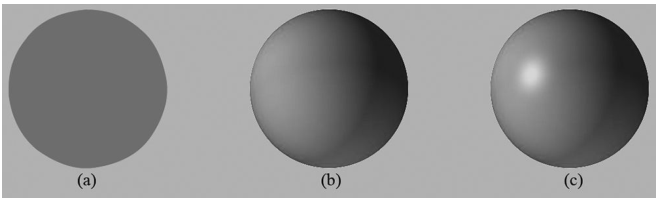
\includegraphics[width=\textwidth]{8-21}
    \centering
    \caption{(a)仅用环境光着色的球体,均匀地照亮它。(b)环境光和漫射照明相结合。 由于朗伯余弦定律,现在从明亮到黑暗平稳过渡。(c)环境光,漫反射光和镜面光。 镜面反射照明产生镜面反射。}
\end{figure}

\begin{flushleft}
NOTICE: 公式8.4是一种常见且流行的照明方程,但它只是一个模型。还有其他照明模型。
\end{flushleft}

%------- 8.9 ---------------
\section{实现材质(Implementing Materials)}
\begin{flushleft}
材质数据结构如下,其定义在 d3dUtil.h 中:\\
\end{flushleft}

\begin{lstlisting}
// Simple struct to represent a material for our demos.  
// A production 3D engine would likely create a class 
// hierarchy of Materials.
struct Material
{
    // Unique material name for lookup.
    std::string Name;

    // Index into constant buffer corresponding to this material.
    int MatCBIndex = -1;

    // Index into SRV heap for diffuse texture.
    int DiffuseSrvHeapIndex = -1;

    // Index into SRV heap for normal texture.
    int NormalSrvHeapIndex = -1;

    // Dirty flag indicating the material has changed and
    // we need to update the constant buffer.
    // Because we have a material constant buffer for each 
    // FrameResource, we have to apply the
    // update to each FrameResource.  Thus, when we modify 
    // a material we should set 
    // NumFramesDirty = gNumFrameResources so that each frame 
    // resource gets the update.
    int NumFramesDirty = gNumFrameResources;

    // Material constant buffer data used for shading.
    DirectX::XMFLOAT4 DiffuseAlbedo = { 1.0f, 1.0f, 1.0f, 1.0f };
    DirectX::XMFLOAT3 FresnelR0 = { 0.01f, 0.01f, 0.01f };
    float Roughness = .25f;
    DirectX::XMFLOAT4X4 MatTransform = MathHelper::Identity4x4();
};
\end{lstlisting}

\begin{flushleft}
对真实世界的材料进行建模需要结合为DiffuseAlbedo和FresnelR0设置实际值,以及一些艺术调整。 例如,金属导体吸收进入金属内部的折射光[Möller08],这意味着金属不会有漫反射(即,DiffuseAlbedo将为零)。 然而,为了补偿我们没有进行100%的光照物理模拟,设置不为零的低DiffuseAlbedo值可以提供更好的艺术效果。 重点是:我们将尝试使用物理上真实的材料值,也可以随意调整我们想要的值以求更好的效果(艺术的角度)。\\
在我们的材料数据结构中,粗糙度在$[0,1]$范围内的标准化浮点值中取值。 粗糙度为 0 表示表面非常光滑,粗糙度为 1 表示物理上可能的最粗糙表面。 标准化范围使得更容易编写粗糙度并比较不同材料之间的粗糙度。 例如,粗糙度为0.6的材料的粗糙度是粗糙度为0.3的材料的两倍。 在着色器代码中,我们将使用粗糙度来导出公式\ref{eq.8.4}中使用的指数$m$。 请注意,根据我们对粗糙度的定义,表面的光泽度(shininess)只是粗糙度(roughness)的倒数:$shininess=1-roughness \epsilon [0,1]$。\\

现在的问题是我们应该在什么样的粒度上指定材料值?材料值可能在表面上变化; 也就是说,表面上的不同点可能具有不同的材料值。 例如,考虑如图\ref{fig:8-22}所示的汽车模型,其中框架,窗户,灯光和轮胎以不同方式反射和吸收光线,因此材料值需要在汽车表面上变化。
\end{flushleft}

\begin{figure}[h]
    \label{fig:8-22}
    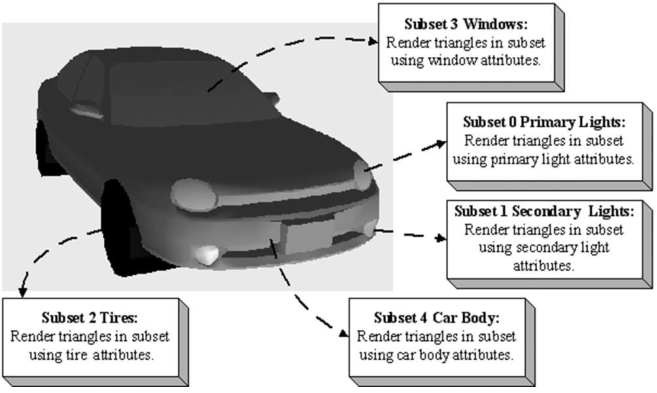
\includegraphics[width=\textwidth]{8-22}
    \centering
    \caption{汽车网格划分为五个材料属性组。}
\end{figure}

\begin{flushleft}
要实现此变化,一种解决方案可能是在每个顶点的基础上指定材质值。 然后,这些每个顶点材质将在光栅化期间在三角形上进行插值,为三角形网格表面上的每个点提供材质值。 然而,正如我们在第7章的“Hills”演示中看到的那样,每个顶点颜色仍然太粗糙,无法逼真地模拟精细细节。 此外,每个顶点颜色会向我们的顶点结构添加额外的数据,我们需要使用工具来绘制每个顶点颜色。 相反,流行的解决方案是使用纹理映射,它必须等到下一章。 对于本章,我们允许在绘制调用频率上进行材料更改。 为此,我们定义每个唯一材料的属性并将它们放在一个表中:\\
\end{flushleft}

\begin{lstlisting}
std::unordered_map<std::string, 
    std::unique_ptr<Material>> mMaterials;
void LitWavesApp::BuildMaterials()
{
    auto grass = std::make_unique<Material>();
    grass->Name = “grass”;
    grass->MatCBIndex = 0;
    grass->DiffuseAlbedo = XMFLOAT4(0.2f, 0.6f, 0.6f, 1.0f);
    grass->FresnelR0 = XMFLOAT3(0.01f, 0.01f, 0.01f);
    grass->Roughness = 0.125f;
    
    // This is not a good water material definition, but
    // we do not have all the rendering tools we need 
    // (transparency, environment reflection), 
    // so we fake it for now.
    auto water = std::make_unique<Material>();
    water->Name = “water”;
    water->MatCBIndex = 1;
    water->DiffuseAlbedo = XMFLOAT4(0.0f, 0.2f, 0.6f, 1.0f);
    water->FresnelR0 = XMFLOAT3(0.1f, 0.1f, 0.1f);
    water->Roughness = 0.0f;

    mMaterials[“grass”] = std::move(grass);
    mMaterials[“water”] = std::move(water);
}
\end{lstlisting}

\begin{flushleft}
上表将材料数据存储在系统内存中。 为了使GPU能够在着色器中访问材料数据,我们需要在常量缓冲区中映射相关数据。 就像我们对每个对象的常量缓冲区一样,我们为每个FrameResource添加一个常量缓冲区,它将存储每个材质的常量:\\
\end{flushleft}

\begin{lstlisting}
struct MaterialConstants
{
    DirectX::XMFLOAT4 DiffuseAlbedo = { 1.0f, 1.0f, 1.0f, 1.0f };
    DirectX::XMFLOAT3 FresnelR0 = { 0.01f, 0.01f, 0.01f };
    float Roughness = 0.25f;
    // Used in the chapter on texture mapping.
    DirectX::XMFLOAT4X4 MatTransform = MathHelper::Identity4x4();
};

struct FrameResource
{
public:
    ...
    std::unique_ptr<UploadBuffer<MaterialConstants>>
    MaterialCB = nullptr;
    ...
};
\end{lstlisting}

\begin{flushleft}
请注意,MaterialConstants结构包含Material数据的子集; 具体来说,它只包含着色器渲染所需的数据。\\
在更新函数中,材料数据随后会被更改(“dirty”)时复制到常量缓冲区的子区域,以便GPU材料常量缓冲区数据与系统内存材料数据保持同步:\\
\end{flushleft}

\begin{lstlisting}
void LitWavesApp::UpdateMaterialCBs(const GameTimer& gt)
{
    auto currMaterialCB = mCurrFrameResource->MaterialCB.get();
    for(auto& e : mMaterials)
    {
        // Only update the cbuffer data if the constants have changed.  
        // If the cbuffer data changes, it needs to be updated 
        // for each FrameResource.
        Material* mat = e.second.get();
        if(mat->NumFramesDirty > 0)
        {
            XMMATRIX matTransform = XMLoadFloat4x4(&mat->MatTransform);

            MaterialConstants matConstants;
            matConstants.DiffuseAlbedo = mat->DiffuseAlbedo;
            matConstants.FresnelR0 = mat->FresnelR0;
            matConstants.Roughness = mat->Roughness;

            currMaterialCB->CopyData(mat->MatCBIndex, matConstants);

            // Next FrameResource need to be updated too.
            mat->NumFramesDirty--;
        }
    }
}
\end{lstlisting}

\begin{flushleft}
现在每个渲染项都包含一个指向材质的指针。 请注意,多个渲染项可以引用相同的Material对象; 例如,多个渲染项可能使用相同的“砖”材质。 反过来,每个Material对象都有一个索引,指定其常量数据是否在材质常量缓冲区中。 从这里,我们可以偏移到我们正在绘制的渲染项所需的常量数据的虚拟地址,并将其设置为期望材质常量数据的根描述符。 (或者,我们可以在堆中偏移到CBV描述符并设置描述符表,但我们在此演示中定义了我们的根签名,以获取材质常量缓冲区而不是表的根描述符。)以下代码显示了我们如何使用不同材质绘制渲染项目:\\
\end{flushleft}

\begin{lstlisting}
void LitWavesApp::DrawRenderItems(
    ID3D12GraphicsCommandList* cmdList, 
    const std::vector<RenderItem*>& ritems)
{
    UINT objCBByteSize = d3dUtil::CalcConstantBufferByteSize(
        sizeof(ObjectConstants));
    UINT matCBByteSize = d3dUtil::CalcConstantBufferByteSize(
        sizeof(MaterialConstants));

    auto objectCB = mCurrFrameResource->ObjectCB->Resource();
    auto matCB = mCurrFrameResource->MaterialCB->Resource();

    // For each render item...
    for(size_t i = 0; i < ritems.size(); ++i)
    {
        auto ri = ritems[i];

        cmdList->IASetVertexBuffers(0, 1, 
            &ri->Geo->VertexBufferView());
        cmdList->IASetIndexBuffer(
            &ri->Geo->IndexBufferView());
        cmdList->IASetPrimitiveTopology(
            ri->PrimitiveType);

        D3D12_GPU_VIRTUAL_ADDRESS objCBAddress = 
            objectCB->GetGPUVirtualAddress() + 
            ri->ObjCBIndex*objCBByteSize;
        D3D12_GPU_VIRTUAL_ADDRESS matCBAddress = 
            matCB->GetGPUVirtualAddress() + 
            ri->Mat->MatCBIndex*matCBByteSize;

        cmdList->SetGraphicsRootConstantBufferView(
            0, 
            objCBAddress);
        cmdList->SetGraphicsRootConstantBufferView(
            1, 
            matCBAddress);

        cmdList->DrawIndexedInstanced(
            ri->IndexCount, 
            1, ri->StartIndexLocation, 
            ri->BaseVertexLocation, 0);
    }
}
\end{lstlisting}

\begin{flushleft}
提醒读者,我们需要在三角形网格表面上的每个点处使用法向量,以便可以确定光线照射到网格表面上的点的角度(对于朗伯余弦定律)。 为了在三角形网格的表面上的每个点处获得近似法向量,我们在顶点级别指定法线。 在光栅化期间,这些顶点法线将在三角形内插值。\\
到目前为止,我们已经讨论过光的成分,但我们还没有讨论过特定类型的光源。 接下来的三节将介绍如何实现灯光,并行灯光,点光源和聚光灯。\\
\end{flushleft}

%------- 8.10 ---------------
\section{平行光(Parallel Lights)}
\begin{flushleft}
平行光(或定向光)近似于非常远的光源。 因此,我们可以将所有入射光线近似相互平行(图\ref{fig:8-23})。 此外,由于光源距离很远,我们可以忽略距离的影响,只需指定光线照射到场景的光强度。
\end{flushleft}

\begin{figure}[h]
    \label{fig:8-23}
    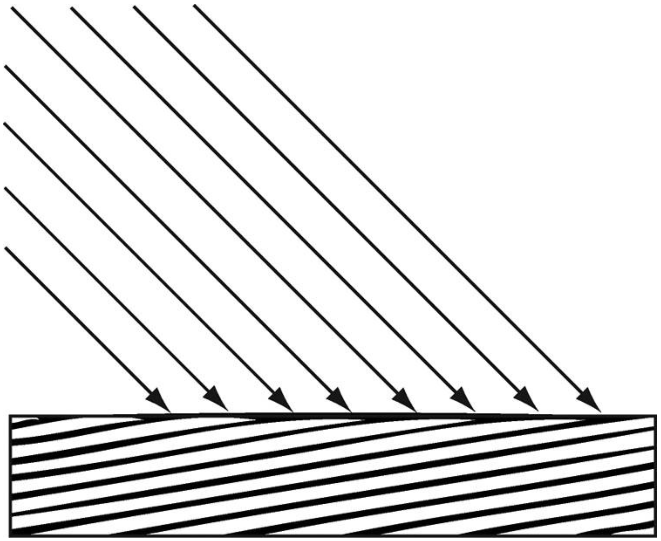
\includegraphics[width=\textwidth]{8-23}
    \centering
    \caption{平行光射入平面}
\end{figure}

\begin{flushleft}
平行光源由向量定义,该向量指定光线行进的方向。 因为光线是平行的,所以它们都使用相同的方向向量。 光向量,瞄准光线行进的相反方向。 可以精确建模为定向光的光源的一个常见例子是太阳(图\ref{fig:8-24})。
\end{flushleft}

\begin{figure}[h]
    \label{fig:8-24}
    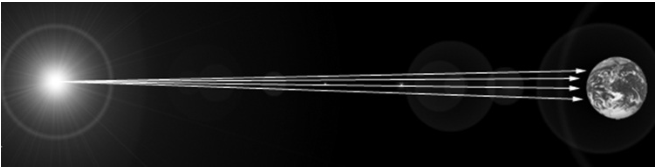
\includegraphics[width=\textwidth]{8-24}
    \centering
    \caption{该图未按比例绘制,但如果您在地球上选择一个小的表面区域,则撞击该区域的光线大致平行。}
\end{figure}

